\documentclass[10pt,a4paper]{article}
\usepackage[UTF8,fontset = windows]{ctex}
\setCJKmainfont[BoldFont=黑体,ItalicFont=楷体]{华文中宋}
\usepackage{amssymb,amsmath,amsfonts,amsthm,mathrsfs,dsfont,graphicx}
\usepackage{ifthen,indentfirst,enumerate,color,titletoc}
\usepackage{tikz}
\usepackage{multicol}
\usepackage{makecell}
\usepackage{longtable}
\usepackage{diagbox}
\usetikzlibrary{arrows,calc,intersections,patterns,decorations.pathreplacing,3d,angles,quotes,positioning,shapes.geometric}
\usepackage[bf,small,indentafter,pagestyles]{titlesec}
\usepackage[top=1in, bottom=1in,left=0.8in,right=0.8in]{geometry}
\renewcommand{\baselinestretch}{1.65}
\newtheorem{defi}{定义~}
\newtheorem{eg}{例~}
\newtheorem{ex}{~}
\newtheorem{rem}{注~}
\newtheorem{thm}{定理~}
\newtheorem{coro}{推论~}
\newtheorem{axiom}{公理~}
\newtheorem{prop}{性质~}
\newcommand{\blank}[1]{\underline{\hbox to #1pt{}}}
\newcommand{\bracket}[1]{(\hbox to #1pt{})}
\newcommand{\onech}[4]{\par\begin{tabular}{p{.9\textwidth}}
A.~#1\\
B.~#2\\
C.~#3\\
D.~#4
\end{tabular}}
\newcommand{\twoch}[4]{\par\begin{tabular}{p{.46\textwidth}p{.46\textwidth}}
A.~#1& B.~#2\\
C.~#3& D.~#4
\end{tabular}}
\newcommand{\vartwoch}[4]{\par\begin{tabular}{p{.46\textwidth}p{.46\textwidth}}
(1)~#1& (2)~#2\\
(3)~#3& (4)~#4
\end{tabular}}
\newcommand{\fourch}[4]{\par\begin{tabular}{p{.23\textwidth}p{.23\textwidth}p{.23\textwidth}p{.23\textwidth}}
A.~#1 &B.~#2& C.~#3& D.~#4
\end{tabular}}
\newcommand{\varfourch}[4]{\par\begin{tabular}{p{.23\textwidth}p{.23\textwidth}p{.23\textwidth}p{.23\textwidth}}
(1)~#1 &(2)~#2& (3)~#3& (4)~#4
\end{tabular}}
\begin{document}

\begin{enumerate}[1.]
%gk10/23
\item 不等式$\frac{2-x}{x+4}>0$的解集是\blank{50}.
\item 若复数$z=1-2\mathrm{i}$($\mathrm{i}$为虚数单位), 则$z\cdot \overline z+z=$\blank{50}.
\item 动点$P$到点$F(2,0)$的距离与它到直线$x+2=0$的距离相等, 则$P$的轨迹方程为\blank{50}.
\item 行列式$\begin{vmatrix} \cos \dfrac{\pi }3 & \sin \dfrac{\pi }6 \\ \sin \dfrac{\pi }3 & \cos \dfrac{\pi }6 \end{vmatrix}$的值是\blank{50}.
\item 圆$C:x^2+y^2-2x-4y+4=0$的圆心到直线l:$3x+4y+4=0$的距离$d=$\blank{50}.
\item 随机变量$\xi$的概率分布率由下表给出: 
\begin{center}
\begin{tabular}{|c|c|c|c|c|}
\hline
$x$ & $7$ & $8$ & $9$ & $10$ \\ \hline
$P(\xi=x)$ & $0.3$ & $0.35$ & $0.2$ & $0.15$ \\ \hline
\end{tabular}
\end{center}
则随机变量$\xi$的均值是\blank{50}.
\item $2010$年上海世博会园区每天$9:00$开园, $20:00$停止入园. 在下面的框图中, $S$表示上海世博会官方网站在每个整点报道的入园总人数, $a$表示整点报道前$1$个小时内入园人数, 则空白的执行框内应填入\blank{50}.
\begin{center}
\begin{tikzpicture}[>=latex, node distance = 3ex]
\node [draw, rounded corners] (start) {开始};
\node [draw, below=of start]  (step1)  {$T\leftarrow 9$, $S\leftarrow 0$};
\node [draw, trapezium, trapezium right angle = 120, below=of step1]  (step2)  {输出$T,S$};
\node [draw, diamond, aspect = 3, below= of step2] (step3) {$T\le 19$};
\node [draw, below= of step3] (step4) {$T\leftarrow T+1$};
\node [draw,  trapezium, trapezium right angle = 120, below = of step4] (step5) {输入$a$};
\node [draw, below = of step5] (step6) {\phantom{$S\leftarrow S+a$}};
\node [right = of step3] (anchor2) {};
\node [below = of step6] (anchor3) {};
\node [draw, below = of anchor3] (end) {结束};
\node [left = of step3] (anchor1) {};
\draw[->] (start)  -- (step1);
\draw[->] (step1)  -- (step2);
\draw[->] (step2)  -- (step3);
\draw[->] (step3)  -- node[right] {是}(step4) ;
\draw[->] (step4)  -- (step5);
\draw[->] (step5)  -- (step6);
\draw[->] (step6) -- (anchor1|-step6) -- (anchor1|-step2) -- (step2);
\draw[->] (step3) --node[above] {否} (anchor2|-anchor2) -- (anchor2|-anchor3) -- (anchor3|-anchor3) -- (end);
\end{tikzpicture}
\end{center}
\item 对任意不等于$1$的正数$a$, 函数$f(x)=\log_a(x+3)$的反函数的图像都经过点$P$, 则点$P$的坐标是\blank{50}.
\item 从一副混合后的扑克牌($52$张)中随机抽取$1$张, 事件$A$为``抽得红桃K'', 事件$B$为``抽得为黑桃'', 则概率$P(A\cup B)=$\blank{50}.(结果用最简分数表示)
\item 在$n$行$n$列矩阵$\begin{pmatrix}
1 & 2 & 3 & \cdots &  n-2 & n-1 & n  \\ 2 & 3 & 4 & \cdots &  n-1 & n & 1  \\ 3 & 4 & 5 & \cdots &  n & 1 & 2  \\ \cdots &  \cdots &  \cdots &  \cdots  & \cdots &  \cdots &  \cdots   \\ n & 1 & 2 & \cdots &  n-3 & n-2 & n-1  \end{pmatrix}$中, 记位于第$i$行第$j$列的数为$a_{ij}$($i,j=1,2\cdots ,n$). 当$n=9$时, $a_{11}+a_{22}+a_{33}+\cdots +a_{99}=$\blank{50}.
\item 将直线$l_1:nx+y-n=0$、$l_2:x+ny-n=0$($n\in \mathbf{N}^*$, $n\ge 2$)$x$轴、$y$轴围成的封闭图形的面积记为$S_n$, 则$\displaystyle\lim_{n\to\infty} S_n=$\blank{50}.
\item 如图所示, 在边长为$4$的正方形纸片$ABCD$中, $AC$与$BD$相交于$O$, 剪去$\triangle AOB$, 将剩余部分沿$OC$、$OD$折叠, 使$OA$、$OB$重合, 则以$A(B)$、$C$、$D$、$O$为顶点的四面体的体积为\blank{50}.
\begin{center}
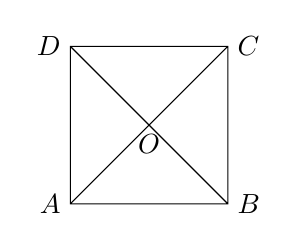
\begin{tikzpicture}[>=latex]
\draw (0,0) -- (2,2) (0,2) -- (2,0) (0,0) rectangle (2,2);
\draw (0,0) node [left] {$A$} coordinate (A);
\draw (2,0) node [right] {$B$} coordinate (B);
\draw (2,2) node [right] {$C$} coordinate (C);
\draw (0,2) node [left] {$D$} coordinate (D);
\draw (1,1) node [below] {$O$} coordinate (O);
\end{tikzpicture}
\end{center}
\item 如图所示, 直线$x=2$与双曲线$\Gamma :\dfrac{x^2}4-y^2=1$的渐近线交于$E_1$, $E_2$两点, 记$\overrightarrow{OE_1}=\overrightarrow{e_1}$, $\overrightarrow{OE_2}=\overrightarrow{e_2}$, 任取双曲线$\Gamma$上的点$P$, 若$\overrightarrow{OP}=a\overrightarrow{e_1}+b\overrightarrow{e_2}$($a,b\in \mathbf{R}$), 则$a$、$b$满足的一个等式是\blank{50}.
\begin{center}
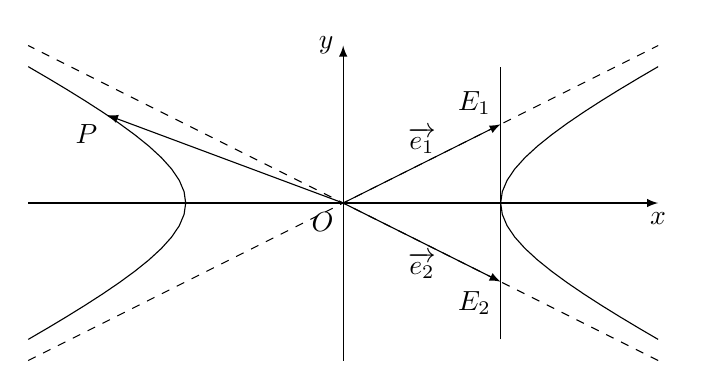
\begin{tikzpicture}[>=latex]
\draw [->] (-4,0) -- (4,0) node [below] {$x$};
\draw [->] (0,-2) -- (0,2) node [left] {$y$};
\draw (0,0) node [below left] {$O$};
\draw [dashed] (-4,-2) -- (4,2) (4,-2) -- (-4,2);
\draw [domain = {-sqrt(3)}:{sqrt(3)}] plot ({2*sqrt(1+pow(\x,2))},\x);
\draw [domain = {-sqrt(3)}:{sqrt(3)}] plot ({-2*sqrt(1+pow(\x,2))},\x);
\draw (2,{-sqrt(3)}) -- (2,{sqrt(3)});
\draw (2,1) node [above left] {$E_1$} coordinate (E1);
\draw (2,-1) node [below left] {$E_2$} coordinate (E2); 
\draw [->] (0,0) -- node [above] {$\overrightarrow{e_1}$} coordinate (e1) (E1);
\draw [->] (0,0) -- node [below] {$\overrightarrow{e_2}$} coordinate (e1) (E2);
\draw (-3,{sqrt(5/4)}) node [below left] {$P$} coordinate (P);
\draw [->] (0,0) -- (P);
\end{tikzpicture}
\end{center}
\item 在集合$U=\{a,b,c,d\}$的子集中选出$2$个不同的子集, 需同时满足以下两个条件: \textcircled{1} $a$、$b$都要选出; \textcircled{2} 对选出的任意两个子集$A$和$B$, 必有$A\subseteq B$或$B\subseteq A$, 那么共有\blank{50}种不同的选法.
\item ``$x=2k\pi +\dfrac{\pi }4$($k\in \mathbf{Z}$)''是``$\tan x=1$''成立的\bracket{20}.
\twoch{充分不必要条件}{必要不充分条件}{充分条件}{既不充分也不必要条件}
\item 直线$l$的参数方程是$\begin{cases} x=1+2t, \\ y=2-t, \end{cases}$($t\in \mathbf{R}$), 则$l$的方向向量是$\overrightarrow d$可以是\bracket{20}.
\fourch{$(1, 2)$}{$(2, 1)$}{$(-2, 1)$}{$(1, -2)$}
\item 若$x_0$是方程$(\dfrac 12)^x=x^{\frac 13}$的解, 则$x_0$属于区间\bracket{20}.
\fourch{$(\dfrac 23, 1)$}{$(\dfrac 12, \dfrac 23)$}{$(\dfrac 13, \dfrac 12)$}{$(0, \dfrac 13)$}
\item 某人要制作一个三角形, 要求它的三条高的长度分别为$\dfrac 1{13},\dfrac 1{11},\dfrac 15$, 则此人能\bracket{20}.
\twoch{不能作出这样的三角形}{作出一个锐角三角形}{作出一个直角三角形}{作出一个钝角三角形}
\item 已知$0<x<\dfrac{\pi }2$, 化简:
$\lg (\cos x\cdot \tan x+1-2\sin ^2\dfrac x2)+\lg [\sqrt 2\cos (x-\dfrac{\pi }4)]-\lg (1+\sin 2x)$.
\item 已知数列$\{a_n\}$的前$n$项和为$S_n$, 且$S_n=n-5a_n-85$, $n\in \mathbf{N}^*$.\\
(1) 证明: $\{a_n-1\}$是等比数列;\\
(2) 求数列$\{S_n\}$的通项公式, 并求出$n$为何值时, $S_n$取得最小值, 并说明理由.
\item 如图所示, 为了制作一个圆柱形灯笼, 先要制作$4$个全等的矩形骨架, 总计耗用$9.6$米铁丝, 骨架把圆柱底面$8$等份, 再用$S$平方米塑料片制成圆柱的侧面和下底面(不安装上底面).
\begin{center}
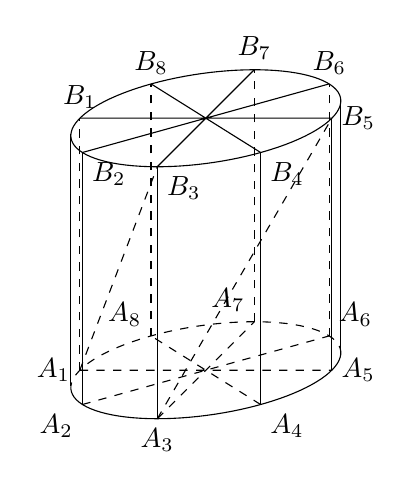
\begin{tikzpicture}[>=latex,scale = 1.6]
\draw [domain = 0:360, samples = 100] plot ({cos(\x)},2,{sin(\x)}); 
\draw ({cos(-atan(sqrt(2)/4))},0,{sin((-atan(sqrt(2)/4)))})  coordinate (R);
\draw [domain = {-atan(sqrt(2)/4)}:{-atan(sqrt(2)/4)+180}, samples = 50] plot ({cos(\x)},0,{sin(\x)}) coordinate (L);
\draw [domain = {-atan(sqrt(2)/4)}:{-atan(sqrt(2)/4)-180}, dashed, samples = 50] plot ({cos(\x)},0,{sin(\x)});
\draw (L) --++ (0,2) (R) --++ (0,2);
\draw ({cos(180)},0,{sin(180)}) node [left] {$A_1$} coordinate (A1);
\draw ({cos(135)},0,{sin(135)}) node [below left] {$A_2$} coordinate (A2);
\draw ({cos(90)},0,{sin(90)}) node [below] {$A_3$} coordinate (A3);
\draw ({cos(45)},0,{sin(45)}) node [below right] {$A_4$} coordinate (A4);
\draw ({cos(0)},0,{sin(0)}) node [right] {$A_5$} coordinate (A5);
\draw ({cos(-45)},0,{sin(-45)}) node [above right] {$A_6$} coordinate (A6);
\draw ({cos(-90)},0,{sin(-90)}) node [above left] {$A_7$} coordinate (A7);
\draw ({cos(-135)},0,{sin(-135)}) node [above left] {$A_8$} coordinate (A8);
\draw [dashed] (A1) --++ (0,2) node [above] {$B_1$} coordinate (B1);
\draw (A2) --++ (0,2) node [below right] {$B_2$} coordinate (B2);
\draw (A3) --++ (0,2) node [below right] {$B_3$} coordinate (B3);
\draw (A4) --++ (0,2) node [below right] {$B_4$} coordinate (B4);
\draw (A5) --++ (0,2) node [right] {$B_5$} coordinate (B5);
\draw [dashed] (A6) --++ (0,2) node [above] {$B_6$} coordinate (B6);
\draw [dashed] (A7) --++ (0,2) node [above] {$B_7$} coordinate (B7);
\draw [dashed] (A8) --++ (0,2) node [above] {$B_8$} coordinate (B8);
\draw (B1) -- (B5) (B2) -- (B6) (B3) -- (B7) (B4) -- (B8);
\draw [dashed] (A1) -- (A5) (A2) -- (A6) (A3) -- (A7) (A4) -- (A8);
\draw [dashed] (A1) -- (B3) (A3) -- (B5);
\end{tikzpicture}
\end{center}
(1) 当圆柱底面半径$r$取何值时, $S$取得最大值? 并求出该最大值(结果精确到$0.01$平方米);\\
(2) 在灯笼内, 以矩形骨架的顶点为点, 安装一些霓虹灯, 当灯笼的底面半径为$0.3$米时, 求图中两根直线$A_1B_3$与$A_3B_5$所在异面直线所成角的大小(结果用反三角函数表示).
\item 若实数$x$、$y$、$m$满足$|x-m|>|y-m|$, 则称$x$比$y$远离$m$.\\
(1) 若$x^2-1$比$1$远离$0$, 求$x$的取值范围;\\
(2) 对任意两个不相等的正数$a$、$b$, 证明: $a^3+b^3$比$a^2b+ab^2$远离$2ab\sqrt {ab}$;\\
(3) 已知函数$f(x)$的定义域$D=\{x| x\ne \dfrac{k\pi }2+\dfrac{\pi }4, \ k\in \mathbf{Z}, \ x\in \mathbf{R}\}$.任取$x\in D$, $f(x)$等于$\sin x$和$\cos x$中远离$0$的那个值.写出函数$f(x)$的解析式, 并指出它的基本性质(结论不要求证明).
\item 已知椭圆$\Gamma$的方程为$\dfrac{x^2}{a^2}+\dfrac{y^2}{b^2}=1$($a>b>0$), 点$P$的坐标为$(-a, b)$.\\
(1) 若直角坐标平面上的点$M$、$A(0, -b)$、$B(a, 0)$满足$\overrightarrow{PM}=\dfrac{1}{2}(\overrightarrow{PA}+\overrightarrow{PB})$, 求点$M$的坐标;\\
(2) 设直线$l_1:y=k_1x+p$交椭圆$\Gamma$于$C$、$D$两点, 交直线$l_2:y=k_2x$于点$E$. 若$k_1\cdot k_2=-\dfrac{b^2}{a^2}$, 证明: $E$为$CD$的中点;\\
(3) 对于椭圆$\Gamma$上的点$Q(a \cos\theta , b \sin\theta )$($0<\theta <\pi$), 如果椭圆$\Gamma$上存在不同的两点$P_1$、$P_2$满足$\overrightarrow{PP_1}+\overrightarrow{PP_2}=\overrightarrow{PQ}$, 写出求作点$P_1$、$P_2$的步骤, 并求出使$P_1$、$P_2$存在的$\theta$的取值范围.


\end{enumerate}
\iffalse















\fi

\end{document}